\clearpage
\subsection{ツェナーダイオード定電圧回路の実験}
\subsubsection{ツェナーダイオード定電圧回路の実験器具}
使用した実験器具を\wtab{kigu3}に示す.
\begin{table}[h]
  \centering
  \caption{実験装置}
  \label{tab:kigu3}
  \scalebox{0.9}{
  \begin{tabular}{cccccc}
	\hline
	機器名&製造元&型番&シリアル番号(または管理番号)\\
	\hline
	ダイオード&不明&1N4736A&不明\\
	直流電源&YOKOGAWA&PA1811&L96-000668\\
	直流用電圧計&YOKOGAWA&YAS 1991&71 BA0 3371\\
	ミリアンペア直流用電流計&YOKOGAWA&YES 1990&70 BA0 1812\\
	可変抵抗器&TOKUSHU DENKI KOGYOSHO&S-3&3201\\
	\hline
  \end{tabular}
}
\end{table}

\subsubsection{ツェナーダイオード定電圧回路の実験方法}
\begin{enumerate}[(1)]
	\item \wfig{zenerc-2}のように回路を構築する.なお,ダイオード$ZD$は1N4736Aを使用した.
\begin{figure}[h]
	\centering
	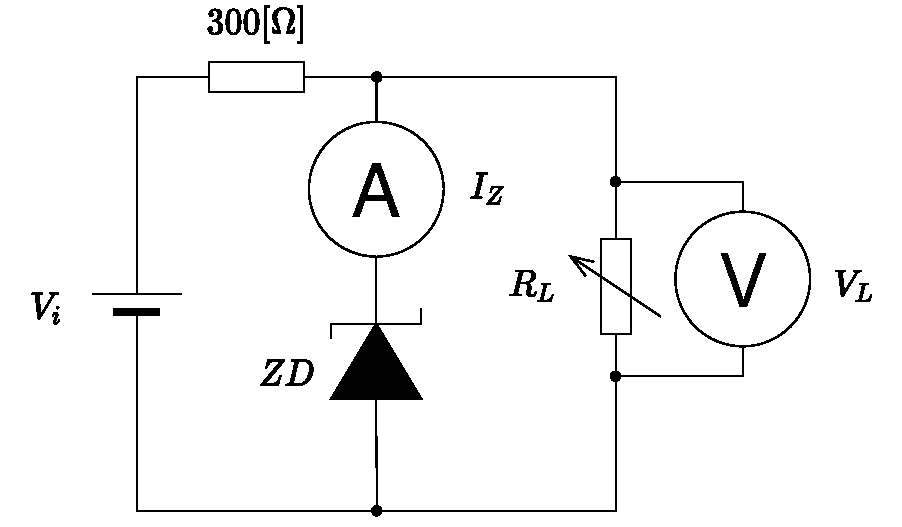
\includegraphics[scale=0.65]{./fig/zenerc-2.pdf}
	\caption{ツェナーダイオード定電圧測定回路}
	\label{fig:zenerc-2}
\end{figure}
	\item 入力$V_i$を$15\,\rm{V}$に固定し,可変抵抗$R_{L}$を変化させてツェナー電流$I_Z$を$2\,\rm{mA}$刻みで$2\,\rm{mA}$から$22\,\rm{mA}$まで変化させた.その際,電流計は端子$30\,\rm{mA}$に接続した.
	\item それぞれの場合で,出力電圧$V_L$と,出力電流$I_Z$を計測した.
	\item 上記のデータを元に$I_{Z}-V_{Z}$,$I_Z-I_L$のグラフを作成した.
\end{enumerate}

\subsubsection{ツェナーダイオード定電圧回路の結果}
\begin{itemize}
	\item \wfig{zener-const-1}に$I_{Z}-V_{Z}$,\wfig{zener-const-2}に$I_{Z}-I_{L}$特性グラフを示す.
出力電圧$V_L$はツェナー電流$I_Z$に依存せず,$7\,\rm{V}$付近で一定であった.
また,出力電流$I_{L}$はツェナー電流$I_Z$増加とともにほぼ比例的に減少している.
\begin{figure}[h]
	\centering
	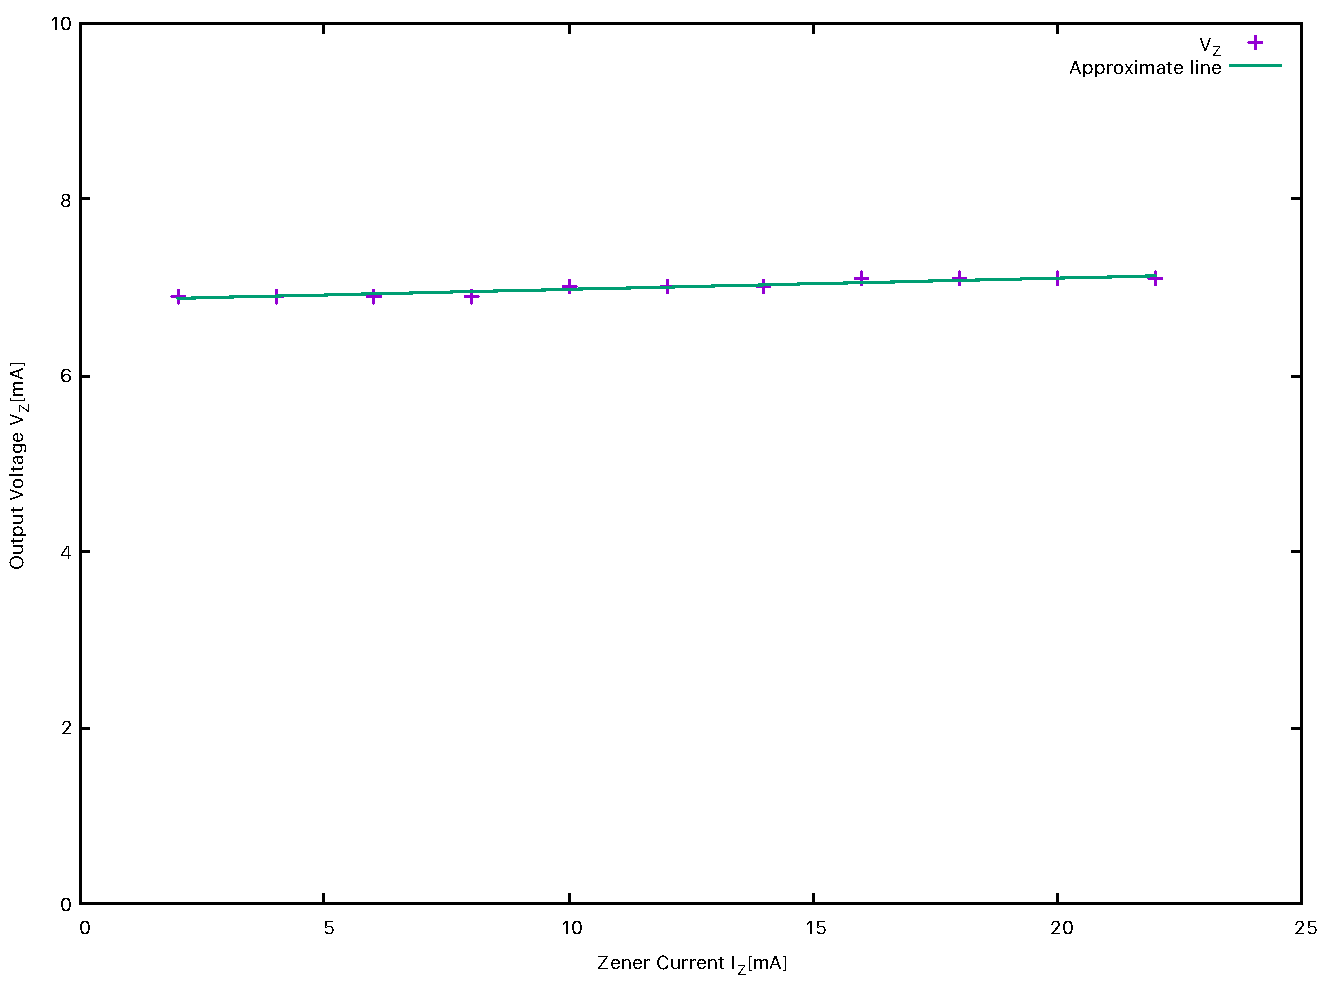
\includegraphics[scale=0.65]{./data/zener/zener-const-1.pdf}
	\caption{定電圧回路の$I_Z-V_Z$特性}
	\label{fig:zener-const-1}
\end{figure}
\begin{figure}[h]
	\centering
	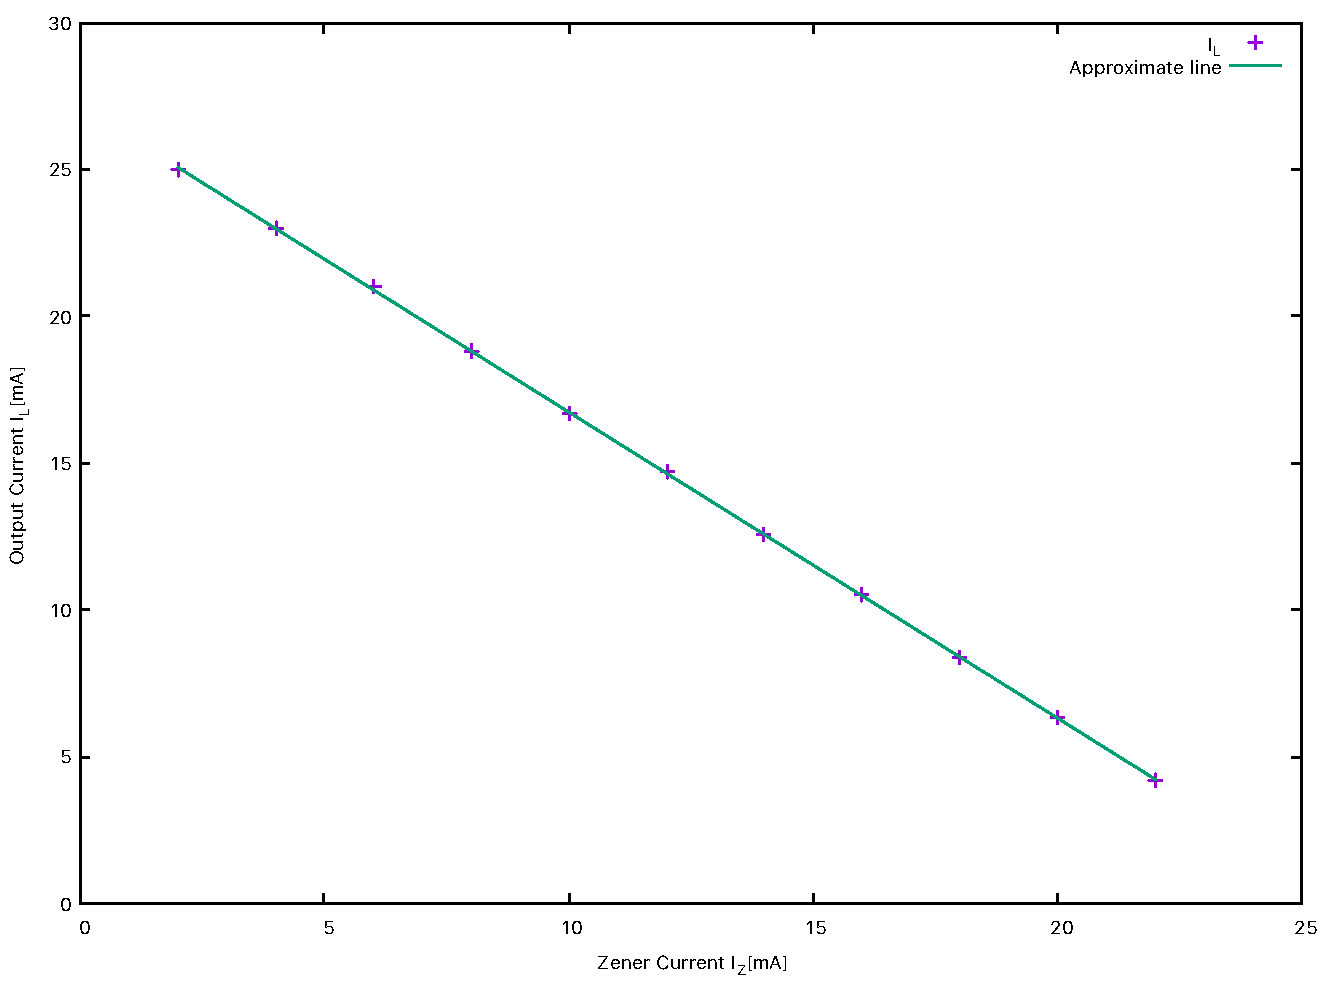
\includegraphics[scale=0.65]{./data/zener/zener-const-2.pdf}
	\caption{定電圧回路の$I_Z-I_L$特性}
	\label{fig:zener-const-2}
\end{figure}
\end{itemize}

\clearpage
\subsubsection{ツェナーダイオード定電圧回路の考察}
\begin{enumerate}[(1)]
	\item 等価回路図(\wfig{zener-eq})を参考にして,測定結果から$R_{L}$,$R_{Z}$,およびこれらの合成抵抗$R_{A}$を算出せよ.
	
	\begin{figure}[h]
	\centering
	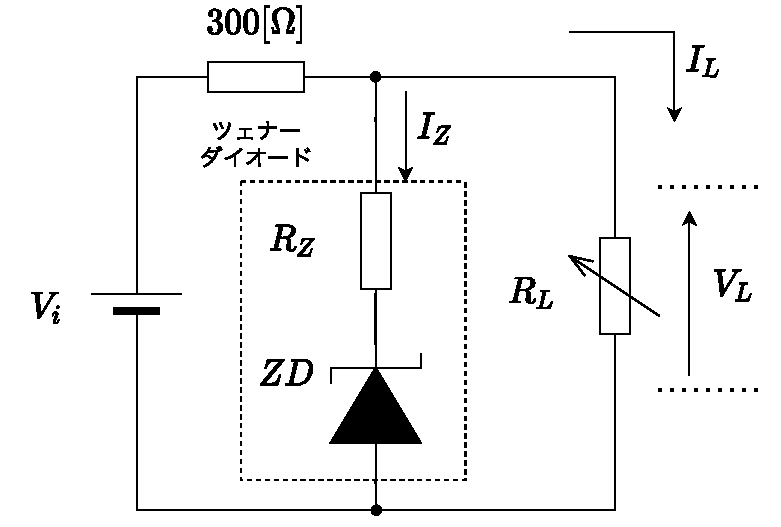
\includegraphics[scale=0.75]{./fig/zener-eq.pdf}
	\caption{ツェナーダイオード定電圧等価回路}
	\label{fig:zener-eq}
	\end{figure}
	\wfig{zener-eq}より,この回路は並列回路であることがわかり,分圧則とオーム則を用いて抵抗値が算出可能である.
	\weq{RL}から\weq{RA}に各抵抗値の導出方法を示す.
\begin{align}
	R_{L}&=\frac{V_{L}}{I_{L}}\label{eq:RL}\\
	R_{Z}&=\frac{V_{L}}{I_{Z}}\label{eq:RZ}\\
	R_{A}&=300+\frac{R_{Z}\cdot 1.0\times 10^{3}}{R_{Z}+1.0\times 10^{3}}\label{eq:RA}
\end{align}
	これらの計算を各ツェナー電流ごとに行なったものを\wtab{rtab}に示す.
	
\begin{table}[h]
\centering
\caption{電流,電圧値により算出した各抵抗値}
\label{tab:rtab}
\scalebox{1.0}{
\begin{tabular}{cccc}
	\hline
	ツェナー電流$I_{Z}$[$\rm{mA}$] & 可変抵抗値$R_{L}$[$\Omega$] & ダイオード抵抗値$R_{Z}$[$\Omega$] & 合成抵抗$R_{A}$[$\Omega$]  \\
	\hline
	 2     & 0.276 & 3.450    & 0.256 \\
	 4     & 0.300 & 1.725    & 0.256 \\
	 6     & 0.329 & 1.150    & 0.256 \\
	 8     & 0.367 & 0.863    & 0.257 \\
	10    & 0.419 & 0.700    & 0.262 \\
	12    & 0.476 & 0.583    & 0.262 \\
	14    & 0.556 & 0.500    & 0.263 \\
	16    & 0.676 & 0.444    & 0.268 \\
	18    & 0.845 & 0.394    & 0.269 \\
	20    & 1.127 & 0.355    & 0.270 \\
	22    & 1.690 & 0.323    & 0.271 \\
	\hline
\end{tabular}
}
\end{table}
この表より,合成抵抗$R_{A}$はほとんどツェナー電流に依存せずに一定の値をとっていることがわかる.このことは,\weq{ZL}で右辺の項が定数のため,左辺の電流値も定数となることとも一致する.
\begin{equation}
	I_{Z}+I_{L}=\frac{V_{i}-V_{L}}{300}
	\label{eq:ZL}
\end{equation}
\begin{figure}[h]
	\centering
	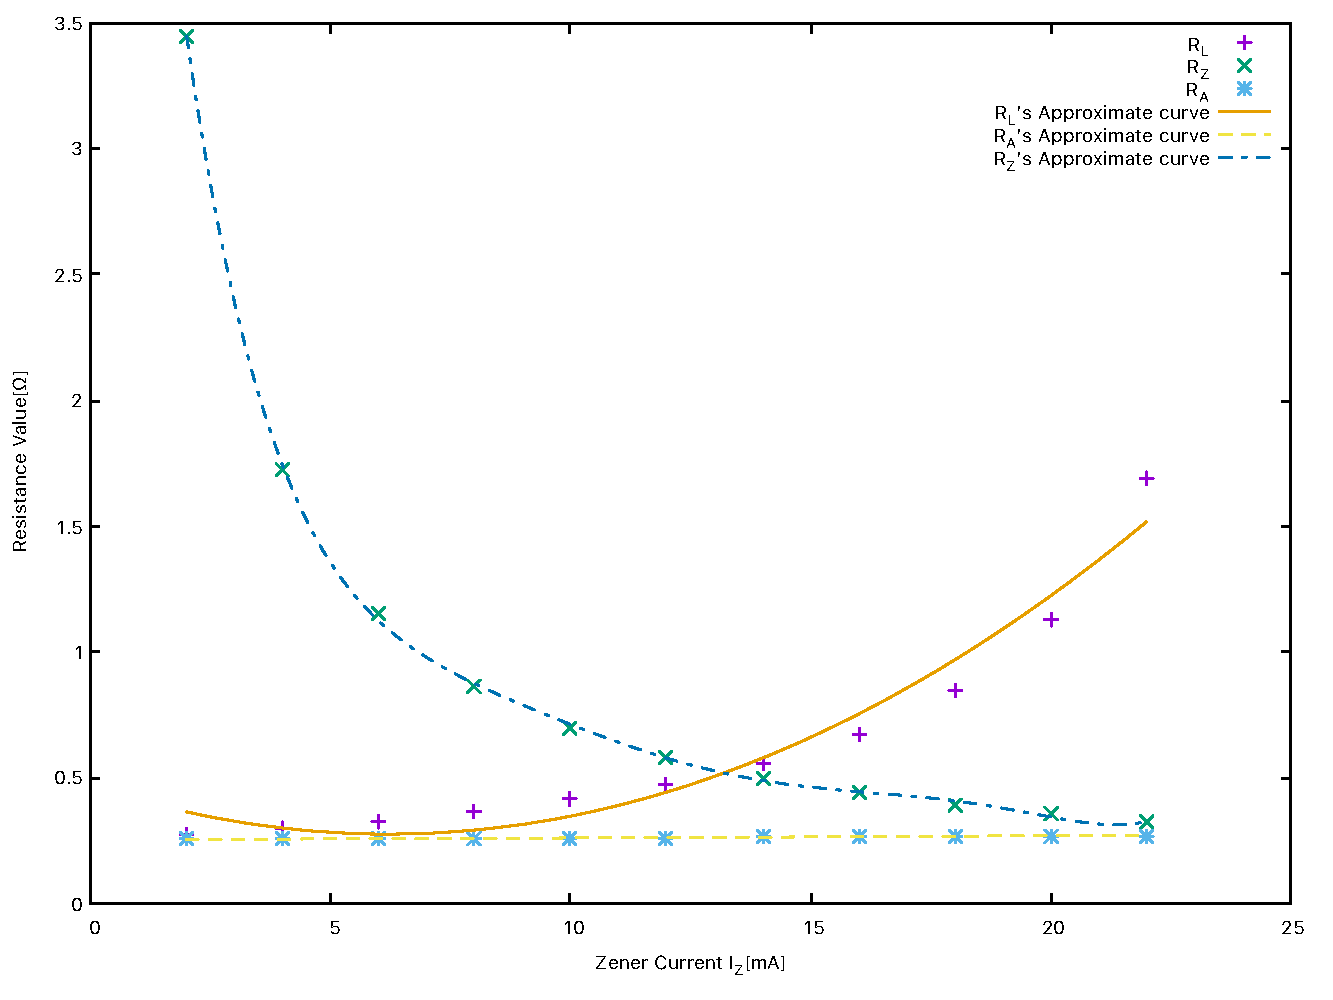
\includegraphics[scale=0.7]{./data/zener/r.pdf}
	\caption{各抵抗のツェナー電流特性}
	\label{fig:rgraph}
\end{figure}
	\item $I_{Z}-R_{L}$特性,$I_{Z}-R_{Z}$特性を同一グラフに重ねて描き,考察せよ.ここで,何について論じたいかを明確にした上で記述すること.

	\wfig{rgraph}は上記式により導出した各抵抗値のツェナー電流特性である.
	合成抵抗はツェナー電流の変化に依存していないが,$R_{L}$は$I_{Z}$に比例し,$R_{Z}$は反比例していることが読み取れる.これは上の考察と矛盾がない.
\end{enumerate}